\section{Airport Air-Pollutant Layer}
\label{sec:air}

NOx, CO and HC are recalculated from representative aircraft--engine combinations in the ICAO
Engine Emissions Databank \citep{icaoeedb}. The mapping is complete for the commercial fleet,
but every row is marked imputed because aircraft registrations and actual engine fits are not
available. The turboprop fallback and fuel-based SO2, PM2.5 and black-carbon factors are
reported separately \citep{emep2023aviation}.

These remain LTO mass estimates rather than a complete airport micro-inventory. Standard fleet
shares stand in for airport-specific aircraft assignments, and actual taxi time, APU, ground
support, brake and tyre sources are not estimated. Consequently the layer supports screening
and method development, not claims about population exposure. A defensible airport inventory
will require registration-to-engine matching and observed times in mode as recommended by ICAO
Doc~9889 \citep{icao9889}.

\begin{figure}[htbp]
\centering
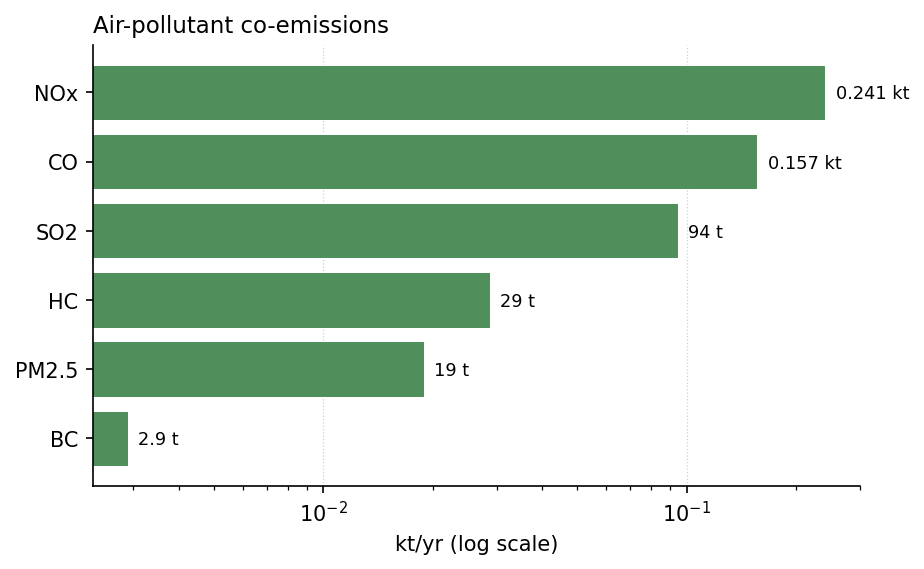
\includegraphics[width=\linewidth]{aviation_air.png}
\caption{Domestic main-engine LTO pollutants on a logarithmic mass axis. Values use
representative, explicitly imputed aircraft--engine mappings.}
\label{fig:air}
\end{figure}
